En la Figura~\ref{fig:diagrama_electronico} se muestra el diagrama electrónico del sistema propuesto, donde se pueden observar los principales componentes y sus conexiones.

\begin{figure}[H]
    \centering
    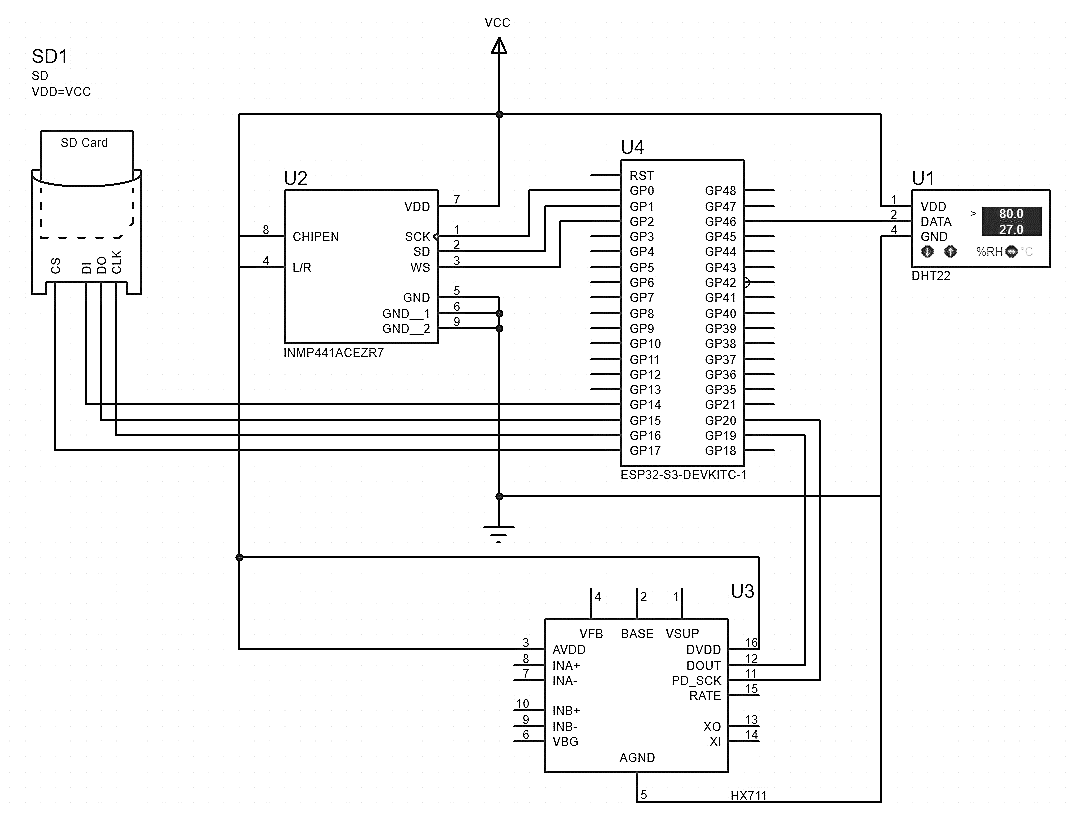
\includegraphics[width=0.9\textwidth]{assets/cap_3/diagrama_electronico.png}
    \caption{Diagrama electrónico del sistema.}
    \label{fig:diagrama_electronico}
\end{figure}

En la figura \ref{fig:diagrama_electronico} se observan los siguientes componentes:
\begin{itemize}
    \item \textbf{Sensor de temperatura y humedad DHT22, U1}: Mide la temperatura y la humedad del ambiente dentro de la colmena.
    \item \textbf{Micrófono INMP441, U2}: Micrófono digital que captura el sonido de la colmena, con una frecuencia de muestreo de 48 kHz, 24 bits y 2 canales, permitiendo el análisis acústico.
    \item \textbf{Interfaz para celdas de carga HX7111, U3}: Mide el peso de la colmena utilizando celdas de carga, proporcionando datos precisos sobre la producción de miel.
    \item \textbf{Microcontrolador ESP32, U4}: Actúa como el cerebro del sistema, encargado de procesar los datos y controlar los demás componentes.
    \item \textbf{Modulo de almacenamiento SD, SD1}: Permite almacenar los datos recolectados por el sistema, como las lecturas de temperatura, humedad, peso y audio.
\end{itemize}